
\documentclass{article}% use option titlepage to get the title on a page of its own.
\usepackage{cite}
\usepackage{listings}
\usepackage{color}
\usepackage{graphicx}
\usepackage{enumitem}


\definecolor{dkgreen}{rgb}{0,0.6,0}
\definecolor{gray}{rgb}{0.5,0.5,0.5}
\definecolor{mauve}{rgb}{0.58,0,0.82}

\lstset{frame=tb,
  language=Python,
  aboveskip=3mm,
  belowskip=3mm,
  showstringspaces=false,
  columns=flexible,
  basicstyle={\small\ttfamily},
  numbers=none,
  numberstyle=\tiny\color{gray},
  keywordstyle=\color{blue},
  commentstyle=\color{dkgreen},
  stringstyle=\color{mauve},
  breaklines=true,
  breakatwhitespace=true,
  tabsize=3
}
\begin{document}

\begin{titlepage}
	\begin{center}
	\line(1,0) {300} \\
	\huge{\textbf{Optimizaci\'on de Flujo en Redes: Reporte 2 }}
	\line(1,0) {300}\\
	
	\textsc{ \Large Mayra Cristina Berrones Reyes}\\ 
	\textsc{\Large Marzo 2018} \\
	\end{center}
\end{titlepage}

\section*{Introducci\'on}

En este reporte lo que se requiere es, tomar los pasos que realizamos en la pr\'actica anterior y re-acomodarlos en forma de clases. Esto nos dar\'a como resultado la primer fase de la pr\'actica, que consiste en realizar un gr\'afo simple. A partir de este nuevo formato, se deber\'an realizar las siguientes funciones para las versiones subsecuentes.

\begin{description}[font=$\bullet$~\normalfont\scshape\color{black}]
\item[\textbf{Gr\'afo normal } ]
\item[\textbf{Gr\'afo dirigido} ]
\item[\textbf{Gr\'afo ponderado}]
\end{description}

\section*{Fase 1: Gr\'afo normal}

El nombre de la clase es $Grafo$. Se importaron las librer\'ias de \textbf{random} y \textbf{math}. Las funciones que contiene esta clase se describen de la siguiente manera.

\begin{lstlisting}
// gr.py
	def __init__(self):

	def puntos(self, num):

	def aristas(self, prob):
	
	def imprimir(self, arch):
	
	def grafica (self):
	
\end{lstlisting}

En la funci\'on $init$ se guardan las variables globales que se utilizan en las dem\'as funciones, ya que no puedes manipular una variable que esta dentro de una funci\'on diferente de la que se este usando actualmente.
\\

Despu\'es est\'a la funci\'on de $puntos$, en la cual se crean la cantidad de puntos aleatorios indicados en la entrada $num$.
\\

En la funci\'on de $aristas$ es donde se crean las conexiones entre los puntos que se crearon en $puntos$. En este caso, el dato de entrada que solicita es el de la probabilidad para que dichos puntos se unan. Entre m\'as grande el n\'umero, m\'as cantidad de conexiones existir\'an.
\\

En la funci\'on $imprimir$ requiere la entrada del nombre del archivo en cual se van a guardar los datos. La terminaci\'on en este ejemplo, es de .dat.
\\

Por \'ultimo, la funci\'on de $grafica$ simplemente se encarga de generar la imagen que ten\'ia de salida el programa de la pr\'actica anterior.

Las lineas necesarias para correr este programa son:

\begin{lstlisting}
// ko.py
from rep2 import Grafo
p = Grafo()
p.puntos(10)
p.aristas(0.5)
p.imprimir("nodos.dat")
p.grafica()
\end{lstlisting}

\begin{figure}[h]

\centering
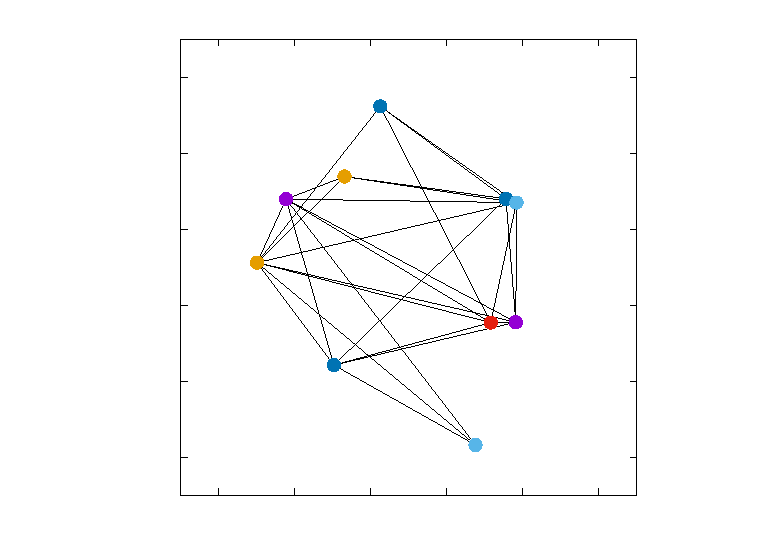
\includegraphics[width = 1\textwidth]{nodos1.eps}
\caption{Gr\'afo normal.}
\end{figure}

\section*{Fase 2: Gr\'afo dirigido}

Para esta secci\'on, se realiz\'o un cambio en la funci\'on de $grafica$, en donde se le agregaron lineas de c\'odigo para especificar la direcci\'on en la que van las aristas hacia los puntos.

\begin{lstlisting}
// gr.py
	def grafica (self, di):
		assert self.archivo is not None
		with open("nodos.plot", 'w') as salida: 
			print('set term eps', file = salida)
			print('set output "nodos.eps"', file = salida)
			print('set size square', file = salida)
			print('set key off', file = salida)
			print ('set xrange [-.1:1.1]', file = salida)
			print ('set yrange [-.1:1.1]', file = salida)
			id = 1
			for i in range(len(self.Ari)):
				if di is 1:
					print('set arrow', id, 'from', self.Ari[i][0], ',', self.Ari[i][1], 'to', self.Ari[i][2], ',', self.Ari[i][3], 'head filled lw 1',  file = salida)
					id +=1
				else:
					print('set arrow', id, 'from', self.Ari[i][0], ',', self.Ari[i][1], 'to', self.Ari[i][2], ',', self.Ari[i][3], 'nohead filled lw 1', file = salida)
					id +=1
			print('plot "nodos.dat" using 1:2:3 with points pt 7 lc var ps 2 ', file = salida)
			print('quit()', file =  salida)
\end{lstlisting}

En los par\'ametros de entrada para la funci\'on, lo que cambia es que ahora se le pide, $1$ en caso de querer un gr\'afo dirigido, y cualquier otro numero en caso de querer un gr\'afo normal. 

\begin{figure}[h]

\centering
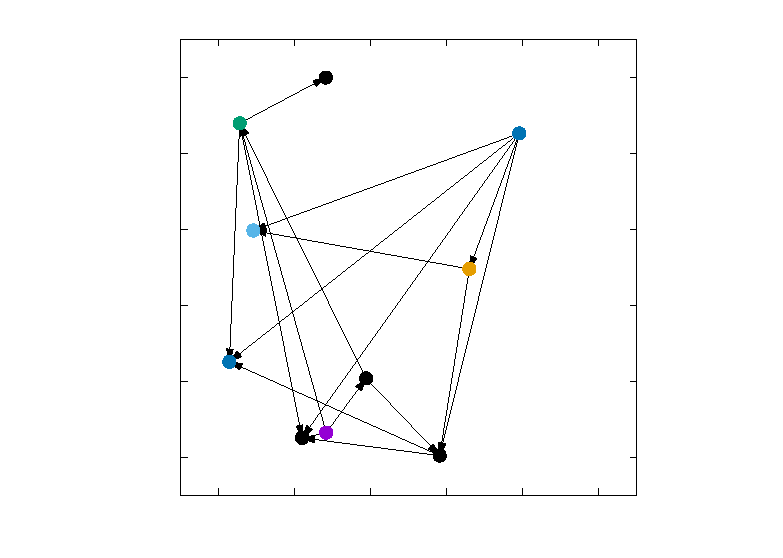
\includegraphics[width = 1\textwidth]{nodo2.eps}
\caption{Gr\'afo dirigido.}
\end{figure}

\section*{Fase 3: Gr\'afo ponderado}

Para esta fase, lo que se requiere es, de alguna manera, darle peso a las aristas que unen los puntos en el gr\'afo. En este caso, se modific\'o tanto la funci\'on de $grafica$ como la de $aristas$. Adem\'as se agreg\'o una variable global para guardar estos datos llamada $pesos$.

Lo que se busca con la variable $pesos$ es calcular la distancia entre los puntos que si se conectan. Entre mas larga sea esta distancia, el costo de recorrerla ser\'a m\'as alto.

\begin{lstlisting}
//rep2.py
	def aristas(self, prob):
		for i in range(self.n - 1):
			self.nodo2.append(self.P[i])
		for i in range(self.n):
			self.nodo3.append(self.P[i])
		for(x1, y1, i) in self.nodo2:
			del self.nodo3[0]
			for(x2, y2, j) in self.nodo3:
				if random() < prob:
					self.Ari.append((x1, y1, x2, y2))
					self.pesos.append((sqrt((x2 - x1) ** 2 + (y2 - y1 )** 2)*100, (x1+x2)/2, (y1+y2)/2))
		print(len(self.Ari))

(...)		
		
	def grafica (self, di):
		assert self.archivo is not None
		with open("nodos.plot", 'w') as salida: 
			print('set term eps', file = salida)
			print('set output "nodos.eps"', file = salida)
			print('set size square', file = salida)
			print('set key off', file = salida)
			print ('set xrange [-.1:1.1]', file = salida)
			print ('set yrange [-.1:1.1]', file = salida)
			id = 1
			for i in range(len(self.Ari)):
				if di is 2 :
					print('set arrow', id, 'from', self.Ari[i][0], ',', self.Ari[i][1], 'to', self.Ari[i][2], ',', self.Ari[i][3], 'head filled lw 1',  file = salida)
					id +=1
				elif di is 1:
					print('set arrow', id, 'from', self.Ari[i][0], ',', self.Ari[i][1], 'to', self.Ari[i][2], ',', self.Ari[i][3], 'nohead filled lw 1', file = salida)
					id +=1
				elif di is 3:
					print('set arrow', id, 'from', self.Ari[i][0], ',', self.Ari[i][1], 'to', self.Ari[i][2], ',', self.Ari[i][3], 'nohead filled lw 1', file = salida)
					print('set label', "'", int(self.pesos[i][0]), "'", 'at', self.pesos[i][1], ',', self.pesos[i][2], file = salida)
					id +=1

			print('plot "nodos.dat" using 1:2:3 with points pt 7 lc var ps 2 ', file = salida)
			print('quit()', file =  salida)
		
\end{lstlisting}

En la entrada de la funci\'on $grafica$, lo que se debe tomar en cuenta es que si se le da un 1, es un gr\'afo simple, si se le da un 2, es un gr\'afo dirigido, y si es un 3, es un gr\'afo ponderado.
\begin{figure}[h]

\centering
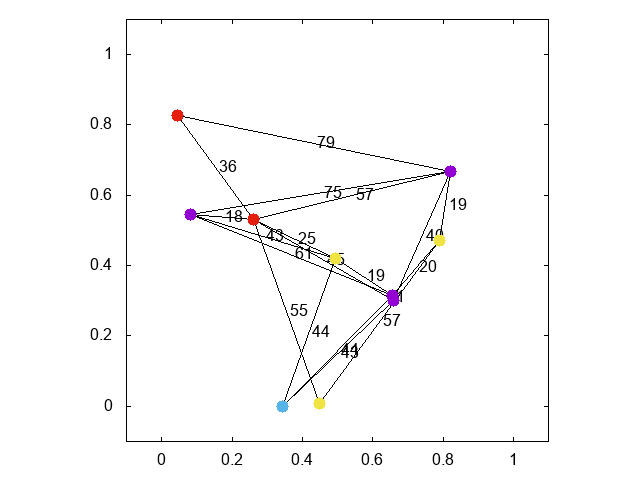
\includegraphics[width = 1\textwidth]{nodos1.png}

\caption{Gr\'afo ponderado.}
\end{figure}

\section*{Conclusi\'on}

Teniendo un buen panorama de estos tres tipos de gr\'afos, podemos empezar a imaginarlos o trasladarlos a los problemas de optimizaci\'on que hemos estado aprendiendo en otras clases, como lo es el del problema del agente viajero. Esta es una de las herramientas que podemos tener para representarlos. Mas adelante, quiz\'a, aprendamos a recorrerlos e intentar encontrar una soluci\'on factible.

\end{document} 












